% =========================================================================== %
% Yes. This is a document.

\documentclass[
	english,
	aspectratio=169,
	table
]{beamer}

% =========================================================================== %
% Theme
\usepackage{scrlfile}
	\ReplacePackage{beamerthemeSHUR}{./sty/beamerthemeSHUR}
	\ReplacePackage{beamerinnerthemefancy}{./sty/beamerinnerthemefancy}
	\ReplacePackage{beamerouterthemedecolines}{./sty/beamerouterthemedecolines}
	\ReplacePackage{beamercolorthemechameleon}{./sty/beamercolorthemechameleon}

\usetheme[
	pageofpages=/,
	bullet=circle,
	titleline=true,
	alternativetitlepage=true,
	watermark="",
	watermarkheight=0px,
	watermarkheightmult=0
	]
{SHUR}

% =========================================================================== %
% the usual stuff

\usepackage[utf8]{inputenc}
\usepackage[T1]{fontenc}
\usepackage{babel}
\usepackage{lmodern}
\usepackage{microtype}
\usepackage{csquotes}

\usepackage{tabularx}
\usepackage{booktabs}
\usepackage{multirow}

\usepackage{color, colortbl}
\usepackage{xcolor}
	\definecolor{tabhighlight}{RGB}{230,240,255}
	\definecolor{tabcontrast} {RGB}{200,210,255}

\usepackage{tabto}
\usepackage{xspace}

% math
\usepackage{amsmath}
\usepackage{amssymb}
\usepackage{dsfont}
\usepackage[arrowdel]{physics}
\usepackage{mathtools}
\usepackage{siunitx}

\usepackage{minted}
	\usemintedstyle{friendly}

\usepackage{tikz}
	\usetikzlibrary{positioning}
	\usetikzlibrary{matrix}
	\usetikzlibrary{shapes.geometric}
	\usetikzlibrary{backgrounds}
	\usetikzlibrary{calc}
	\usetikzlibrary{decorations.pathreplacing}
	\tikzstyle{every picture}+=[remember picture] 
\usepackage{adjustbox}

\usepackage[most]{tcolorbox}
	\tcbsetforeverylayer
		{colback=cyan!10!white,
		 colframe=cyan!75!black,
		 arc=0pt,
		 outer arc=0pt,
		 parbox=false
		}
	\newtcolorbox{codebox}[1][Code]
		{colback=black!5!white,
		 colframe=blue!40!black,
		 title=#1,
		 leftupper=6mm
		}
	\newtcolorbox{cmdbox}[1][Kommandozeilen-Befehl]
		{colback=black,
		 coltext=white,
		 fontupper=\ttfamily ,
		 colframe=blue!40!black,
		 title=#1,
		 outer arc=0pt,
		 leftupper=2mm
		}
	\newtcolorbox{warnbox}[1][Beachte]
		{colback=black!5!white,
		 colframe=red!40!black,
		 title=#1
		}
	\newtcolorbox{hintbox}[1][Tipp]
		{colback=black!5!white,
		 colframe=green!40!black,
		 parbox=false,
		 title=#1
		}
	\newenvironment{itembox}
		{\begin{tcolorbox}\begin{itemize}}%
		{\end{itemize}\end{tcolorbox}}
	\newtcolorbox{doublebox}[1][.3]
		{righthand width=#1\linewidth,
		 sidebyside,
		 sidebyside gap=6mm,
		 sidebyside align=center,
		 lower separated=false}
	
%==============================================================================%
% GLOBAL MACROS

\newcommand*{\eg}{e.\,g. }
\newcommand*{\ie}{i.\,e. }

\newcommand{\Thus}{\ensuremath{\Rightarrow}\xspace}
\newcommand{\thus}{\ensuremath{\rightarrow}\xspace}

\newcommand*{\tabcrlf}{\\ \midrule}			% actually still allows for optional argument

\newcommand*{\inPy}[1]{\mintinline{python3}{#1}}

% =========================================================================== %

\author{Stefan Hartinger}
\title{Python for Scientific Applications}
\subtitle{Part 11: Parallel Programming}
\institute{University of Regensburg, department for theoretical physics}
\date{Summer Term 2021}

% =========================================================================== %

\begin{document}
% =========================================================================== %

\begin{frame}[t,plain]
\titlepage
\end{frame}

% =========================================================================== %\\

\begin{frame}{Simultaneous}
%
\begin{columns}[T]
\column{.5\linewidth}
\begin{center}
	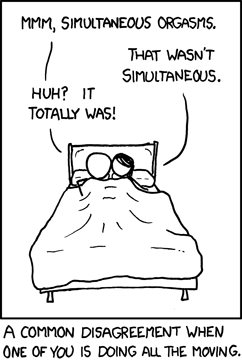
\includegraphics[width=.55\linewidth]{./gfx/xkcd-simultaneous}
\end{center}
%
\column{.5\linewidth}
\begin{center}

\end{center}
\begin{center}
	\emph{I'm leaving you for your twin. He's more mature than you by now.}
	
	\vspace{12pt}
	Source: \url{https://xkcd.com/514/}
\end{center}
\end{columns}
%
\end{frame}

% =========================================================================== %\\

\begin{frame}{Two Scenarios}
%
\begin{columns}[T]
\column{.5\linewidth}
CPU-bound problems
\begin{itemize}
\item Have a large number $N$ of similar computations to do
	\begin{itemize}
	\item Different input, same steps for each input
	\end{itemize}
\item Independent from another
	\begin{itemize}
	\item Solution of problem A does not depend on state/solution of B
	\end{itemize}
\item Combined runtime $N \times t(\text{problem})$ is too long
\end{itemize}
%
\column{.5\linewidth}
I/O-bound problems
\begin{itemize}
\item Want to respond to user input while waiting for a device
\item Think of a hard disk, network service, ...
\item CPU is not (overly) busy but waits for the device
\item Code becomes unresponsive while waiting for the device
\end{itemize}
\end{columns}

\vspace{12pt}
\begin{columns}[T]
\column{.5\linewidth}
\Thus Multiprocessing
%
\column{.5\linewidth}
\Thus Multithreading
\end{columns}
%
\end{frame}

% =========================================================================== %

\begin{frame}{Vocabulary}
%
\begin{columns}[T]
\column{.5\linewidth}
Processes
\begin{itemize}
\item Full \enquote{infrastructure} for running code
	\begin{itemize}
	\item Own memory (\ie independent variables)
	\item Own process ID (\ie known to the OS)
	\end{itemize}
\item Takes a little to set up
\item Communication between processes possible but not trivial
\end{itemize}
%
\column{.5\linewidth}
Threads
\begin{itemize}
\item Lightweight variant of process
\item Shared memory, no own process ID
	\begin{itemize}
	\item Easier communication
	\item Race conditions everywhere
	\end{itemize}
\item Python: all threads run on the same CPU!
\item No true parallel computing, only switching from task to task
\end{itemize}
\end{columns}
%
\begin{center}
\emph{Unfortunately, Python's use of the word \emph{thread} is different from what is meant in other languages}
\end{center}
%
\end{frame}

% =========================================================================== %\\

\begin{frame}[fragile]{Race Conditions}
%
\begin{columns}[T]
\column{.5\linewidth}
\begin{itemize}
\item Think of 2+ routines running \emph{in parallel}
\item Shared ressource \texttt{x} (\eg a variable)
\item Routine A wants to read \texttt{x}
\item Routine B wants to write \texttt{x}
\item Who goes first?
\item Even more problematic: \texttt{x} is a composite structure (\eg a \inPy{class} instance)
\item[\Thus] Need to implement locks (aka mutexes: mutual exclusion)
\end{itemize}
%
\column{.5\linewidth}
\begin{center}
	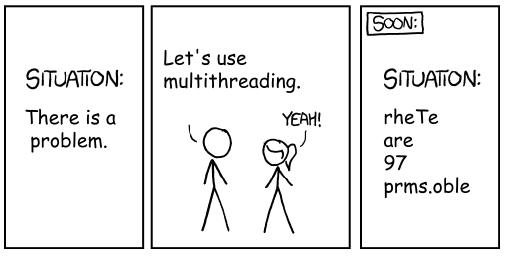
\includegraphics[width=\linewidth]{./gfx/reddit-xkcd-multithreading}
	{\tiny
	 Source: \url{https://www.reddit.com/r/ProgrammerHumor/comments/dtiufv/multithreading_fixing_a_problem/}
	 
	 Basen on: \url{https://xkcd.com/927/}
	}
\end{center}
\end{columns}

\vspace{6pt}
Note: Python multiprocessing saves you \emph{some} race condition trouble, but not all of it.
%
\end{frame}

% =========================================================================== %

\begin{frame}[fragile]{Multiprocessing}
%
\begin{itemize}
\item Load module \texttt{multiprocess} (pre-installed)
\item Write one or several normal subroutines (\inPy{def subroutine(*args, **kwargs)})
\item Usually no return value
	\begin{itemize}
	\item There's a way to make use of return values. Unfortunately we don't have the time for that
	\end{itemize}
\item Define 
\begin{minted}{python3}
proc = Process(
    target = subroutine,
    args   = tupleOfPositionalArguments,
    kwargs = dictOfKeywordArgs
)
\end{minted}
\item Call \texttt{proc.start()} to make the process run (\enquote{asynchronously})
\item Call \texttt{proc.join()} to wait untill the process has finished
	\begin{itemize}
	\item Otherwise, processes can become \enquote{zombies}
	\end{itemize}
\end{itemize}
%
\end{frame}

% =========================================================================== %

\begin{frame}[fragile]
%
\begin{codebox}[Example: Starting multiple processes]
\begin{minted}[linenos, fontsize=\scriptsize]{python3}
from multiprocessing import Process
import time

def worker (name) :
    print("This is worker ", name, ", beginning to do my job", sep="")
    time.sleep(1)
    print("Worker", name, "has finished doing their job")

processes = []
tic = time.time()
for name in ['Caspar', 'Charlotte', 'Alex', 'Jasmin'] :
    processes.append(Process(target=worker,args=(name,)))
for proc in processes : proc.start()
for proc in processes : proc.join()
toc = time.time()
    
print()
print("All workers have finished their jobs.")
print("Time elapsed:", toc - tic, "seconds")
\end{minted}
\end{codebox}
%
\end{frame}

% =========================================================================== %

\begin{frame}[fragile]
%
\begin{cmdbox}[Possible output: starting multiple processes]
\begin{minted}[fontsize=\scriptsize]{text}
This is worker Caspar, beginning to do my jobThis is worker Charlotte
, beginning to do my jobThis is worker 
Alex, beginning to do my job
This is worker Jasmin, beginning to do my job
Worker WorkerCasparWorkerWorker   has finished doing their job JasminAlexCharlotte
  has finished doing their job 
has finished doing their jobhas finished doing their job


Al workers have finished their jobs.
Time elapsed: 1.0600121021270752 seconds
\end{minted}
\end{cmdbox}

\begin{center}
\Thus A lot of time saved, but results can (will!) interfere with one another!
\end{center}
%
\end{frame}

% =========================================================================== %

\begin{frame}{Locks (aka Mutexes)}
%
\begin{itemize}
\item To avoid interference at critical points: let one process \enquote{own} a critical ressource
\item Object: \inPy{multiprocessing.Lock}
	\begin{itemize}
	\item Object that can only be owned by one process at a time
	\item Makes other (non-owning) processes wait until ressource is free
	\end{itemize}
\item Processes can call method \texttt{acquire}
	\begin{itemize}
	\item Tries to get ownership of lock
	\item If successfull: execute next command
	\item Otherwise (if other process already owns the lock): waits until the other process releases the lock
	\end{itemize}
\item Processes can call method \texttt{release}
	\begin{itemize}
	\item Allow others to acquire the lock
	\end{itemize}
\end{itemize}
%
\end{frame}

% =========================================================================== %

\begin{frame}[fragile]
%
\begin{codebox}[Example: Starting multiple processes with a lock to prevent interference]
\begin{minted}[linenos, fontsize=\scriptsize]{python3}
from multiprocessing import Process, Lock
import time

def worker (name, lock) :
    lock.acquire()
    print("This is worker ", name, ", beginning to do my job", sep="")
    lock.release()
    
    time.sleep(1)
    
    lock.acquire()
    print("Worker", name, "has finished doing their job")
    lock.release()

lock = Lock()
processes = []
for name in ['Caspar', 'Charlotte', 'Alex', 'Jasmin'] :
    processes.append(Process(target=worker,args=(name, lock)))

# ... as before
\end{minted}
\end{codebox}
%
\end{frame}

% =========================================================================== %

\begin{frame}[fragile]
%
\begin{cmdbox}[Possible output: Starting multiple processes with a lock to prevent interference]
\begin{minted}[fontsize=\scriptsize]{text}
This is worker Caspar, beginning to do my job
This is worker Charlotte, beginning to do my job
This is worker Alex, beginning to do my job
This is worker Jasmin, beginning to do my job
Worker Caspar has finished doing their job
Worker Charlotte has finished doing their job
Worker Alex has finished doing their job
Worker Jasmin has finished doing their job

Al workers have finished their jobs.
Time elapsed: 1.0793380737304688 seconds
\end{minted}
\end{cmdbox}

\begin{center}
\Thus Time consuming but uncritical part runs in parallel,\\
	problematic part forced to run sequential.
\end{center}
%
\end{frame}

% =========================================================================== %

\begin{frame}
%
\begin{warnbox}[Deadlocks]
It is possible to write code where process A waits for process B but Process B waits for A. This is called \emph{deadlock}.

\vspace{6pt}
Usually this happens when two locks (or similar mechanisms) are in play.

\vspace{6pt}
If you run into a deadlock: terminate by pressing \texttt{CTRL + C} in the console, or kill the process with your task manager.

\vspace{6pt}
\Thus KISS-principle (keep it simple, stupid): use only one lock mechanism at a time!
\end{warnbox}
%
\end{frame}

% =========================================================================== %

\begin{frame}[fragile]
%
\begin{tcbraster}[raster columns=2,
                  raster equal height,
                  nobeforeafter,
                  raster column skip=0.5cm]
\begin{codebox}[Example: Deadlock]
\begin{minted}[fontsize=\scriptsize, linenos]{python3}
from multiprocessing import Process
from multiprocessing import Lock
import time

def workerA (lockA, lockB) :
    lockA.acquire()
    print("worker A has lock A")
    time.sleep(.1)
    lockB.acquire()
    print("worker A has lock B")
    lockB.release()
    lockA.release()
def workerB (lockA, lockB) :
    lockB.acquire()
    print("worker B has lock B")
    time.sleep(.1)
    lockA.acquire()
    print("worker B has lock A")
    lockB.release()
    lockA.release()
\end{minted}
\end{codebox}
%
\begin{codebox}[(... continued)]
\begin{minted}[fontsize=\scriptsize, linenos, firstnumber=last]{python3}
    
processes = []

lockA = Lock()
lockB = Lock()
processes.append(Process(
    target=workerA,
    args=(lockA, lockB))
)
processes.append(Process(
    target=workerB,
    args=(lockA, lockB))
)

for proc in processes : proc.start()
for proc in processes : proc.join()

print("done")
\end{minted}
\end{codebox}
\end{tcbraster}
%
\end{frame}

% =========================================================================== %

\begin{frame}[fragile]{Communicating between Processes I}
%
\begin{itemize}
\item \texttt{multiprocessing.Value}s
	\begin{itemize}
	\item A single variable
	\item Can be shared between processes
	\item Built-in lock
	\item Fixed data type: \inPy{num = Value('i', 42)} constructs a shareable \inPy{int}
	\item Access via \texttt{num.value}
	\end{itemize}
\item \texttt{multiprocessing.Arrays}s
	\begin{itemize}
	\item C-style array (\ie like in NumPy), can be shared
	\item \inPy{arr = Array('i', range(5))}
	\item Direct access like in a \inPy{list}: \texttt{a[0]} for both, read/write access
	\end{itemize}
\end{itemize}
%
\end{frame}

% =========================================================================== %

\begin{frame}[fragile]{Communicating between Processes II}
%
\begin{itemize}
\item \texttt{multiprocessing.Queue}s
	\begin{itemize}
	\item FIFO -- first in first out
	\item Method \texttt{put} -- like \texttt{append} with \inPy{list}s
	\item Method \texttt{get} -- like \texttt{pop} with \inPy{list}s
	\item Can be used to distribute work over processes while ensuring the same job is not done twice
	\item \texttt{get} \emph{waits} until there is something in the Queue -- deadlocks possible
	\item Possilbe to set a \texttt{timeout} value and a \texttt{maxsize}
	\end{itemize}
\item \texttt{multiprocessing.Pipe}s and \texttt{multiprocessing.Connection}s
	\begin{itemize}
	\item \texttt{Pipe()} returns a \inPy{tuple} of \texttt{Connection}s
	\item Duplex (two way) communication between pairs of processes
	\item Methods \texttt{send} and \texttt{recv} on \texttt{Connection}s
	\item \texttt{recv} \emph{waits} until there is a message in the pipe
	\item Method \texttt{poll} on \texttt{Connection}s asks whether any messages are in the pipe.
	\end{itemize}
\end{itemize}
%
\end{frame}

% =========================================================================== %

\begin{frame}[fragile]
%
\begin{tcbraster}[raster columns=2,
                  raster equal height,
                  nobeforeafter,
                  raster column skip=0.5cm]
\begin{codebox}[Example: Producer-Consumer]
\begin{minted}[fontsize=\scriptsize, linenos]{python3}
from multiprocessing import Process, \
    Queue, Value, Lock
import time

def producer (ID, queue, stop, lock) :
    lock.acquire()
    print("producer", ID,
          "begins production")
    lock.release()
    
    while not stop.value :
        lock.acquire()
        print("producer", ID,
              "produces goods")
        lock.release()
        
        time.sleep(.1)
        queue.put(
            f"stuff from producer #{ID}"
        )
\end{minted}
\end{codebox}
%
\begin{codebox}[(... continued)]
\begin{minted}[fontsize=\scriptsize, linenos, firstnumber=last]{python3}
def consumer (ID, queue, stop, lock) :
    lock.acquire()
    print("consumer", ID,
          "begins consumption")
    lock.release()
    
    while not stop.value :
        time.sleep(.2)
        msg = f"consumer {ID} "
        if queue.empty() :
            msg += "takes a day off."
        else :
            msg += "consumes " + \
                   queue.get()
        lock.acquire()
        print(msg)
        lock.release()
\end{minted}
\end{codebox}
\end{tcbraster}
%
\end{frame}

% =========================================================================== %

\begin{frame}[fragile]
%
\begin{tcbraster}[raster columns=2,
                  raster equal height,
                  nobeforeafter,
                  raster column skip=0.5cm]
\begin{codebox}[(... continued)]
\begin{minted}[fontsize=\scriptsize, linenos, firstnumber=last]{python3}
lock        = Lock()
queue       = Queue()
stop        = Value('b', False)
nProducers  =  5
nConsumers  = 10
worktime    =  5

processes = []
for i in range(nProducers) :
    processes.append(Process(
        target=producer,
        args=(i, queue, stop, lock)
    ))

for i in range(nConsumers) :
    processes.append(Process(
        target=consumer,
        args=(i, queue, stop, lock)
    ))
\end{minted}
\end{codebox}
%
\begin{codebox}[(... continued)]
\begin{minted}[fontsize=\scriptsize, linenos, firstnumber=last]{python3}
    
for p in processes :
    p.start()
    
time.sleep(worktime)
stop.value = True

for p in processes :
    p.join()

print("unconsumed goods:",
      queue.qsize()
)
\end{minted}
\end{codebox}
\end{tcbraster}
%
\end{frame}

% =========================================================================== %

\begin{frame}{Threads}
%
\begin{itemize}
\item Same concepts -- different package
\item \inPy{import threading}
\item Use \texttt{Lock}, \texttt{Queue}, ... from \texttt{threading}, not from \texttt{multiprocessing}!
\item Multiprocessing can be used instead of Threads!
\item The inverse is not true.
\end{itemize}
%
\end{frame}

% =========================================================================== %

\begin{frame}[fragile]{So much more to say -- Links}
%
\begin{itemize}
\item Multiprocessing
	\begin{itemize}
	\item Full docs: \url{https://docs.python.org/3/library/multiprocessing.html}
	\item Brief overview: \url{https://tutorialedge.net/python/python-multiprocessing-tutorial/}
	\item In depth tutorial: \url{https://zetcode.com/python/multiprocessing/}
	\end{itemize}
\item Threading
	\begin{itemize}
	\item Full docs: \url{https://docs.python.org/3/library/threading.html}
	\item Brief overview: \url{https://tutorialedge.net/python/python-multithreading-tutorial/}
	\item In depth tutorial: \url{https://realpython.com/intro-to-python-threading/}
	\end{itemize}
\item On both techniques
	\begin{itemize}
	\item Actually, there's even more than \texttt{multiprocessing} and \texttt{threading} ...
	\item \url{https://realpython.com/python-concurrency/}
	\end{itemize}
\end{itemize}
%
\end{frame}
\end{document}

% MAREI!!
% whom do I give credit? Where?